\chapter{Appendices} \label{appendix}

\section{Estimated Timeline}
By the beginning of the Fall'09 semester, I plan to design a taxonomy and implement a low-level software process events abstraction into symbolic representation. The database schema will be extended for storing these data and indexes. Immediately after that, I will proceed with the implementation of fundamental algorithms for associated and sequential patterns mining. This new data model and KDD toolkit will allow me to discover more low-level behavior patterns some of which might be found useful though the empirical evaluation during the period of data collection from the Fall'09 Software engineering class. I will be working with those students who will demonstrate a relevant recurrent behavior in the software process for clarification of observed phenomena.

By the end of the Spring'10 semester I am planning to finish all of my experiments and the software system implementation, and will move on to a peer-reviewed publication and the dissertation thesis defense.

\section{Figures}
\begin{figure}[tbp]
   \centering
   \includegraphics[height=200mm]{trajectory_db.eps}
   \caption{The database schema used for the Hackystat Telemetry data retrieval and indexing in the pilot project.}
   \label{fig:trajectory_db}
\end{figure}

\begin{figure}[tbp]
   \centering
   \includegraphics[height=185mm]{distribution.eps}
   \caption{The distribution of the Hackystat Telemetry data. While individual telemetry streams (panel $b$, left three plots for each stream represent raw data, right three plots - Z-normalized data) show different data distributions, the combined and normalized data (panel $a$) close to the normal distribution. Combined data was used for creation of the \textit{Universal Telemetry SAX alphabet}.}
   \label{fig:distribution}
\end{figure}


